\section{Application: Finding completions of under-constrained glassy structures to isostatic}
\label{sec:bodypin}
% \bibliography{paper}

We can use DR-plans to help in solving questions in designs for graphene and silica bi-layers \cite{silica_bilayers} \cite{sructure_of_2d_glass}. Specifically, we will look into the problem when you have a mono-layer and it is under-constrained. Our goal is to make such a layer isostatic. This can be done in a number of ways.

\begin{figure}\centering
    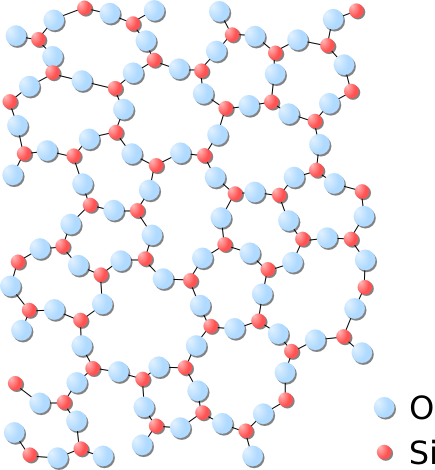
\includegraphics[width=0.4\linewidth]{img/Silica} \hspace{0.5cm}
    \raisebox{0.3\height}{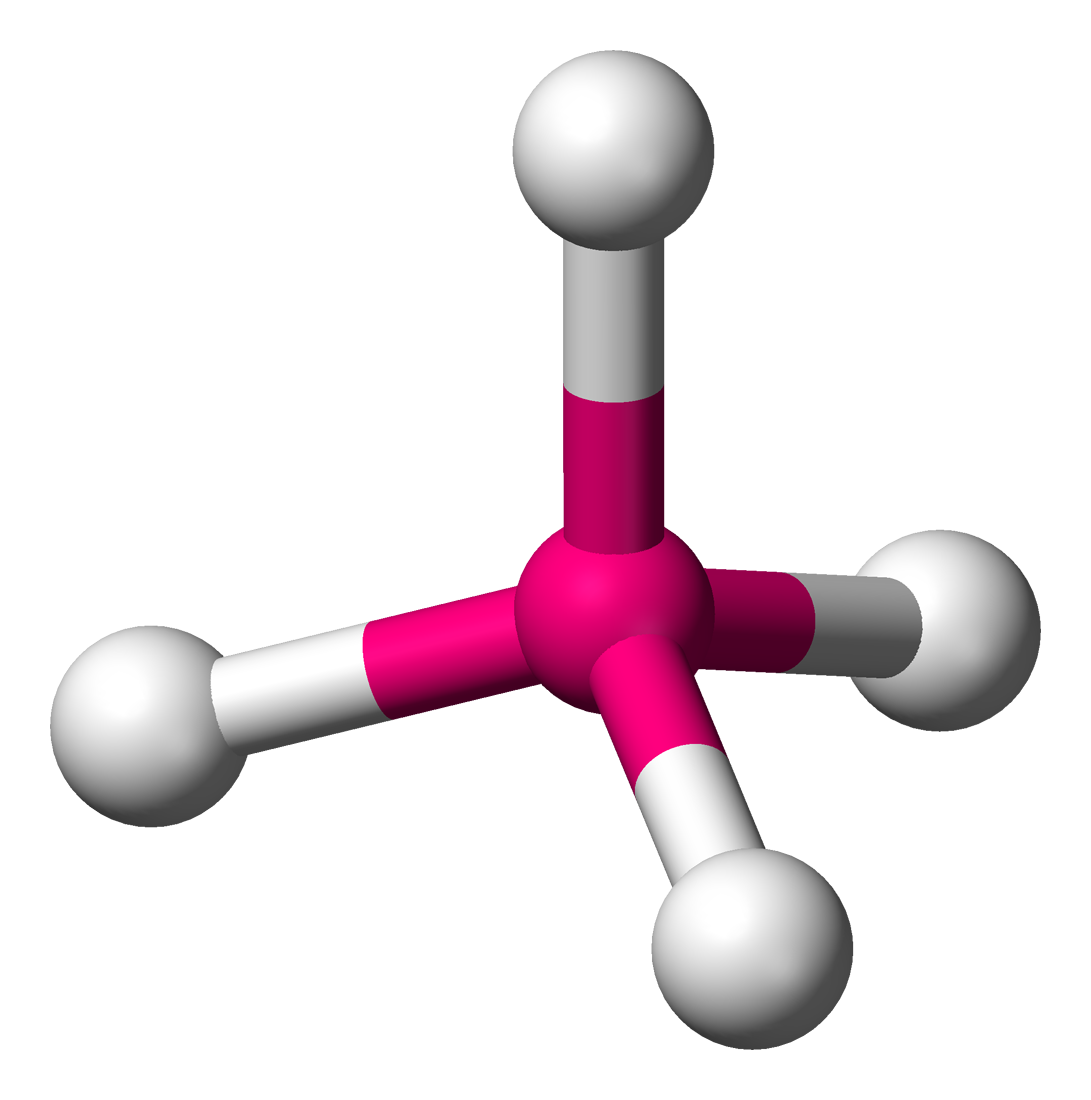
\includegraphics[width=0.2\linewidth]{img/Silicon_tetrahedron}}
    \caption{Example of a single mono-layer of a Silica Oxygen glassy structure. This can be thought of as a multi-triangle-pin qusec where the Silicon atoms are the triangles and the Oxygen atoms are the pins. Not shown here are other layers stacked on this one. Each Silicon atom has the structure seen to the right, and so binds to another Oxygen atom in an adjacent mono-layer. Pictures taken from \cite{silica_figure} and \cite{tetra_silica_figure}.}
    \label{fig:silica_glass}
\end{figure}

\begin{enumerate}
    \item Pin together 2 under-constrained mono-layers in such a way that the resulting bi-layer becomes isostatic (see Figure \ref{fig:silica_glass}).
    \item Pin the boundary in such a way that the resulting system is isostatic.
    \item Build the structures by repeated subdivision to ensure they are isostatic at each layer (see Figure \ref{fig:subdivision})
\end{enumerate}

We will discuss item 2 in detail in this section. In each case, we are specifically interested in how to they can be applied to get a resulting isostatic structure with a small DR-plan, so a realization can be found quickly. To answer these questions, we first introduce the structures we model the problems with:

\begin{figure}\centering
    (a)
    \begin{subfigure}{0.2\linewidth}
        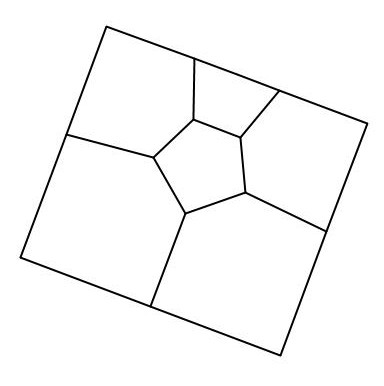
\includegraphics[width=\linewidth]{img/pentl1}
    \end{subfigure}
    %
    $\rightarrow$
    \begin{subfigure}{0.2\linewidth}
        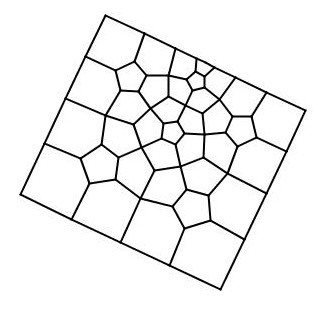
\includegraphics[width=\linewidth]{img/pentl2}
    \end{subfigure}
    %

    (b)
    \begin{subfigure}{0.8\linewidth}
        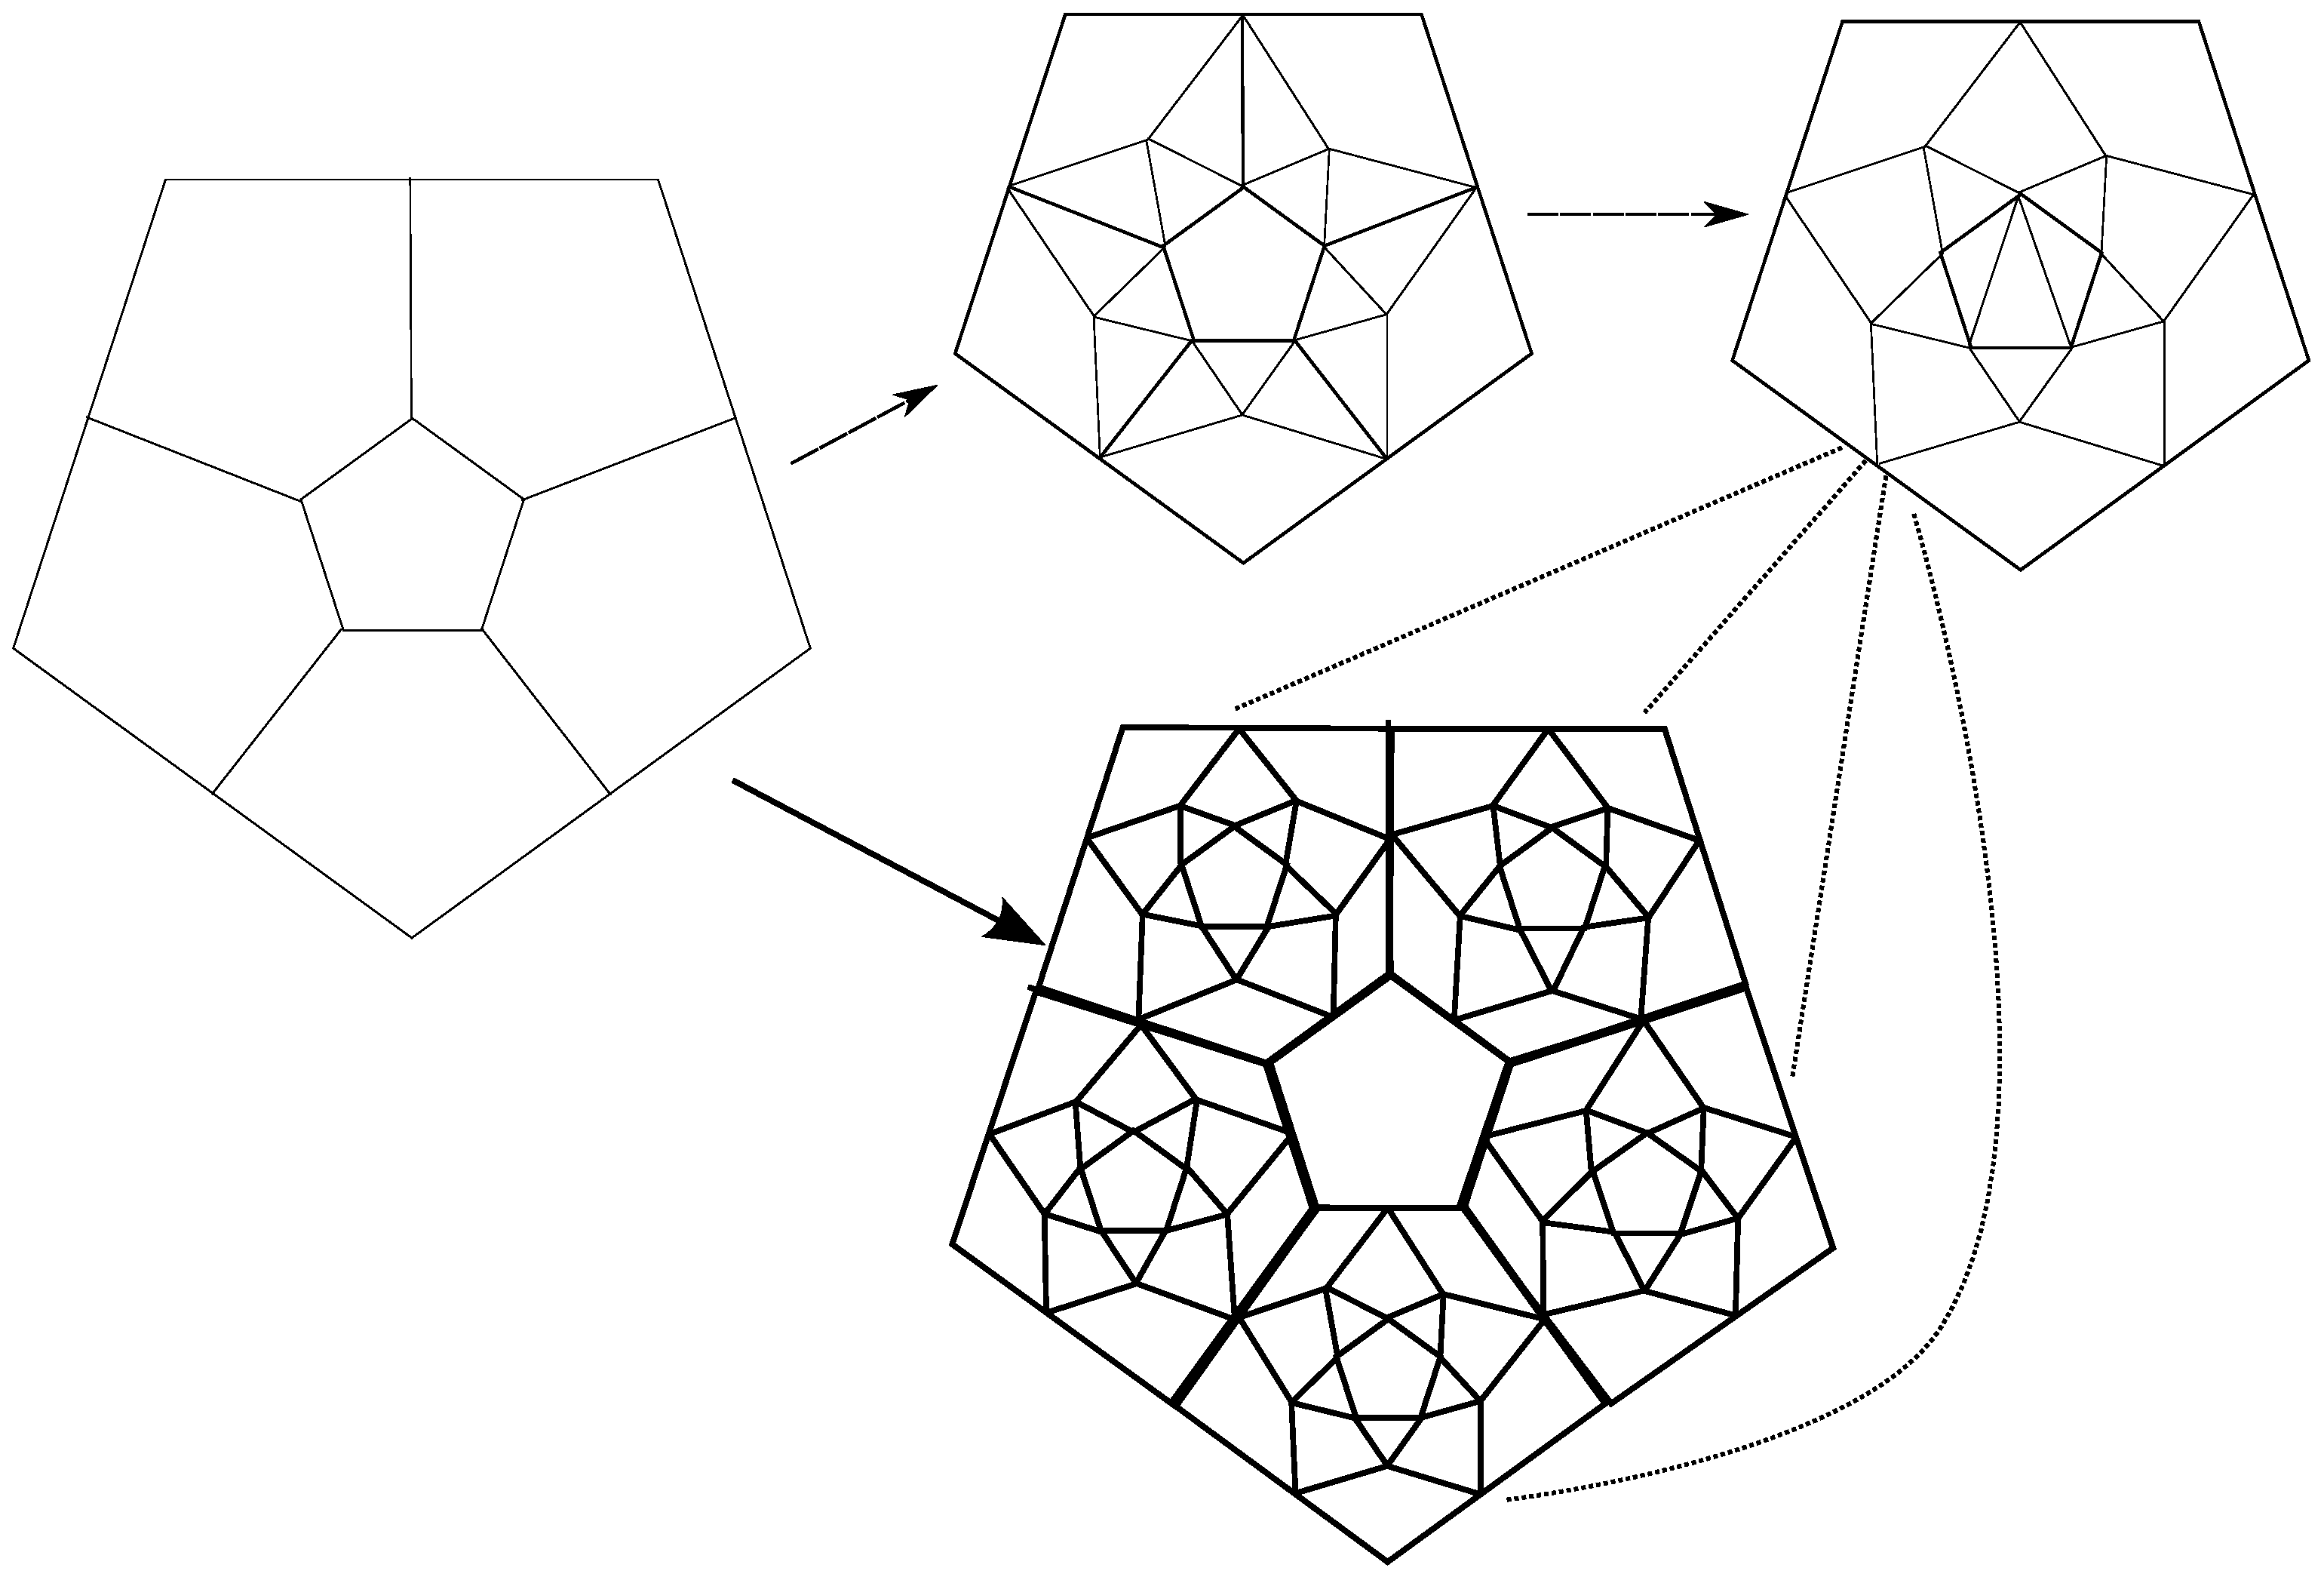
\includegraphics[width=\linewidth]{img/pentawesome}
    \end{subfigure}
    \caption{Examples of self-similarity in the form of repeated subdivision. In (a), a simple subdivision is done that does not guarantee isostatic. In (b), a more complicated scheme is used, ensuring that the resulting graph is both isostatic and non-tree-decomposable. Credit to \cite{subdivision_paper} for (a).}
    \label{fig:subdivision}
\end{figure}

\subsection{Body-Pin}


\begin{definition}
    A \dfn{body-hyperpin qusecs} is a qusecs where the object are rigid bodies that are pinned together by some number of pins.
\end{definition}

\begin{remark}
    A body-hyperpin qusecs is a special case of bar-joint qusecs that we have been studying. As such, the DR-planning discussed in Section \ref{sec:DRP} is unchanged and the work in Section \ref{sec:recomb} will still go through with slight modifications.
\end{remark}

\begin{proof}
    We can replace each body that has only one pin by a single vertex. A body with 2 pins can be replaced by an edge. In general, a body with $n$ pins can be replaced by a 2-tree on $n$ vertices. When looking for a DR-plan, we treat each body as trivial, so they become the leaves of our plan. The optimal completion problem and approach of Section \ref{sec:DRP} are unchanged. The optimal parameterization problem in Section \ref{sec:DRP} now has an additional constraint that all edges in the 2-tree representation of the bodies must be removed together, not individually.
\end{proof}

For the rest of this section, we will only be dealing with the DR-plan  of such qusecs. As such, we will refer only to the underlying graph of the qusecs. We now go over 2 sub-classes of body-hyperpin graphs for modeling Examples 4 and 5 in Section \ref{sec:intro}.

\begin{definition}
\label{def:body-pin}
    A body-pin graph is a body-hyperpin graph with the following conditions:
    \begin{itemize}
        \item Each pin is shared by at most 2 bodies
        \item No 2 bodies share more than one pin
    \end{itemize}
    Such a body-pin graph can also be seen as a \dfn{body-bar graph} where the bodies are the original bodies and each pin represents 2 bars from one body to another. Such body-bar graphs with 1 and 2-dof can be characterized by being $(3,4)$ and $(3,5)$-tight respectively.
\end{definition}

\begin{definition}
    A \dfn{multi-triangle-pin graph} is a body-hyperpin graph where each body is a triangle, meaning it is pinned in at most 3 places. This is also represented as a hyper-graph where each pin is a vertex and each triangle represents a tri-hyperedge. For such hyper-graphs, 1 and 2-dof can be characterized by $(2,4)$ and $(2,5)$-tightness respectively.
\end{definition}

Body-pin graphs are of particular interest to us in the context of Example 4 in Section \ref{sec:intro}. Multi-triangle-pin graphs can be used to represent the silica bi-layers and glassy structures described in Example 5 of Section \ref{sec:intro}, where each triangle is the junction of ``disks'' in the plane (see Figure \ref{fig:silica_glass}). Typically, these systems are not isostatic, so to relate the work of this paper to the systems, we define a slightly different kind of DR-plan:

\begin{definition}
    A \dfn{$(k,l)$-tight DR-plan} is one in which each child node is either a vertex maximal proper $(k,l)$-tight sub-graph of the parent node or it is trivial. In our case, the trivial nodes are just the bodies.
\end{definition}

We can develop the notion of a canonical DR-plan for certain $(k,l)$-tightness conditions similar to the way we did in Section \ref{sec:DRP}.

\begin{observation}
    For the 1-dof body-hyperpin graphs described above, a DR-plan node will follow one of the following:

    \begin{itemize}
        \item Its children will be 2 proper vertex maximal 1-dof graphs that intersect on another 1-dof graph
        \item Its children will be a number of proper maximal 1-dof sub-graphs, joined pairwise by at most one pin
    \end{itemize}
\end{observation}

\begin{proof}
    \todo{Item 1 Follows from paper?}

    For item 2, consider the case where we have more than 2 proper vertex maximal 1-dof sub-graphs $s_1, ..., s_k, k > 2$. Then, if $k_i$ and $k_j$ are joined by $2$ pins, $k_i \cup k_j$ would be $(3,4)$-tight and hence $k_i$ and $k_j$ are not vertex maximal.
\end{proof}

\begin{remark}\label{rem:1dofcanon}
    All $(k,l)$-tight canonical DR-plans are optimal. We can find such a DR-plan in the same time complexity as the $(2,3)$-tight case for bar and joint graphs discussed in Section \ref{sec:DRP}. This is due tot he fact that such $(k,l)$-tight graphs are matroidal and have a pebble game.
\end{remark}

\begin{figure*}\centering
\begin{subfigure}{0.2\linewidth}\centering
    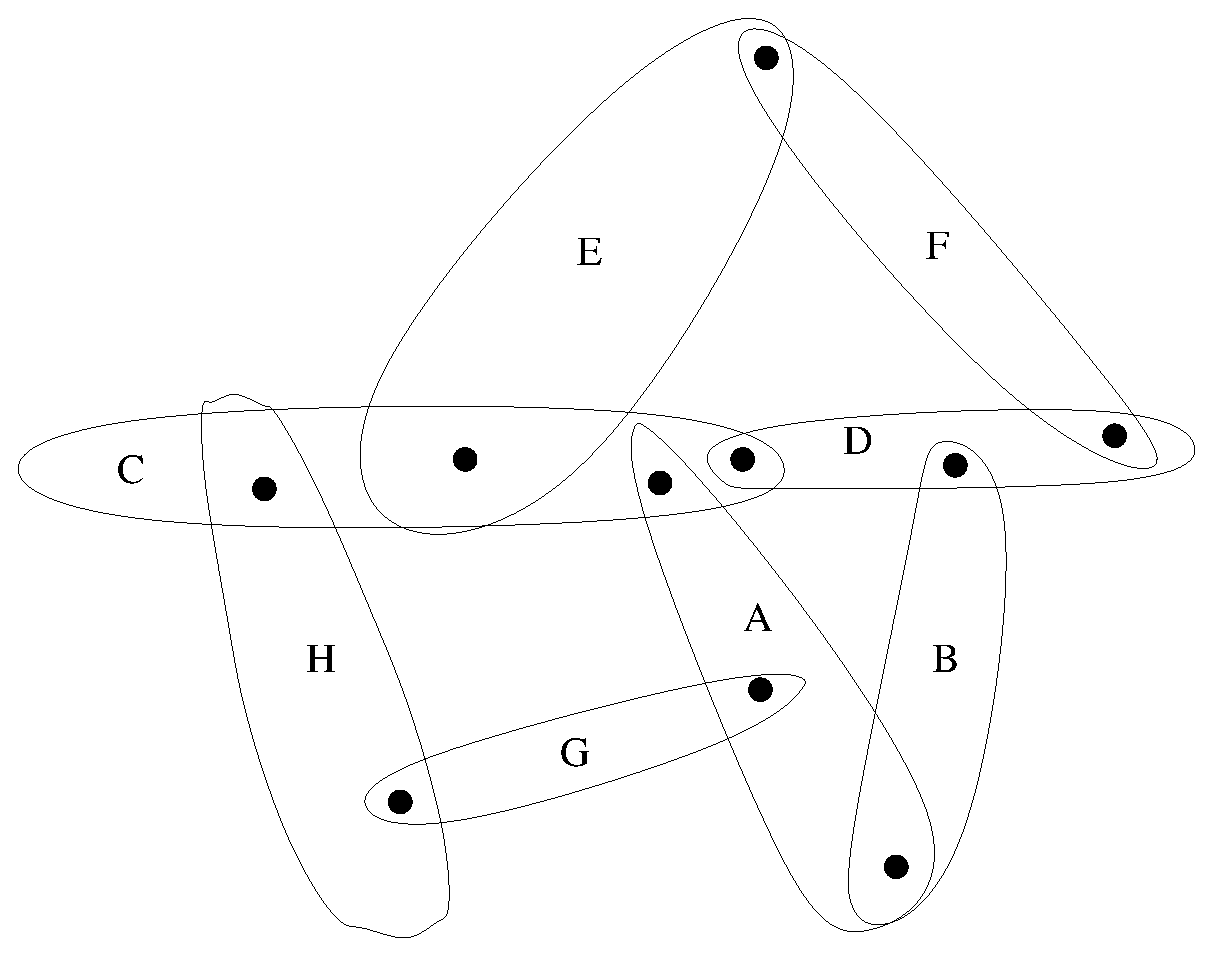
\includegraphics[width=\linewidth]{img/bodypin}
    \caption{}
\end{subfigure}
%
\begin{subfigure}{0.2\linewidth}\centering
    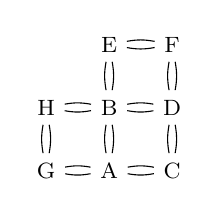
\begin{tikzpicture}[scale=0.8]
    % \tikzstyle{v}=[draw, circle, minimum size=0.1cm, scale=0.7, font=\footnotesize]
    \tikzstyle{v}=[font=\footnotesize]

    \node[v] (a) at (0,0) {A};
    \node[v] (b) at (0,1) {B};
    \node[v] (c) at (1,0) {C};
    \node[v] (d) at (1,1) {D};
    \node[v] (e) at (0,2) {E};
    \node[v] (f) at (1,2) {F};
    \node[v] (g) at (-1,0) {G};
    \node[v] (h) at (-1,1) {H};

    \draw (a) to [bend right=10](b);
    \draw (a) to [bend left=10](b);
    \draw (a) to [bend right=10](c);
    \draw (a) to [bend left=10](c);
    \draw (d) to [bend right=10](c);
    \draw (d) to [bend left=10](c);
    \draw (b) to [bend right=10](d);
    \draw (b) to [bend left=10](d);
    \draw (b) to [bend right=10](e);
    \draw (b) to [bend left=10](e);
    \draw (b) to [bend right=10](h);
    \draw (b) to [bend left=10](h);
    \draw (g) to [bend right=10](h);
    \draw (g) to [bend left=10](h);
    \draw (g) to [bend right=10](a);
    \draw (g) to [bend left=10](a);
    \draw (f) to [bend right=10](e);
    \draw (f) to [bend left=10](e);
    \draw (f) to [bend right=10](d);
    \draw (f) to [bend left=10](d);
\end{tikzpicture}
    \caption{}
\end{subfigure}
%
\begin{subfigure}{0.35\linewidth}\centering\scriptsize
    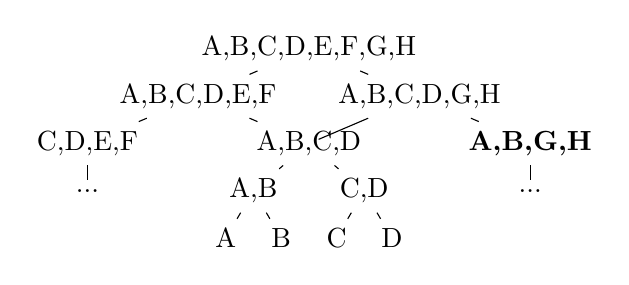
\begin{tikzpicture}
[level 1/.style={sibling distance=8em},
level 3/.style={sibling distance=4em},
level 4/.style={sibling distance=2em}, level distance=0.6cm
]
    \tikzstyle{n}=[draw, fill, circle]

    \node (a) at (0,0) {A,B,C,D,E,F,G,H}
        child { node {A,B,C,D,E,F} 
            child { node {C,D,E,F}
                % child {node { }}
                child {node {...}}
                % child {node { }}
                % child {node { }}
                } 
            child { node[sibling distance=2em] {A,B,C,D}
                child {node {A,B} 
                    child {node {A}}
                    child {node {B}}
                    }
                child {node {C,D}
                    child {node {C}}
                    child {node {D}}
                    }    
                } 
            }
        child { node {A,B,C,D,G,H} 
            child { node { } }
            child { node {{\bf A,B,G,H}} 
                % child {node { }}
                child {node {...}}
                % child {node { }}
                % child {node { }}
            }
        };
\end{tikzpicture}
    \caption{}
\end{subfigure}
%
\begin{subfigure}{0.2\linewidth}\centering
    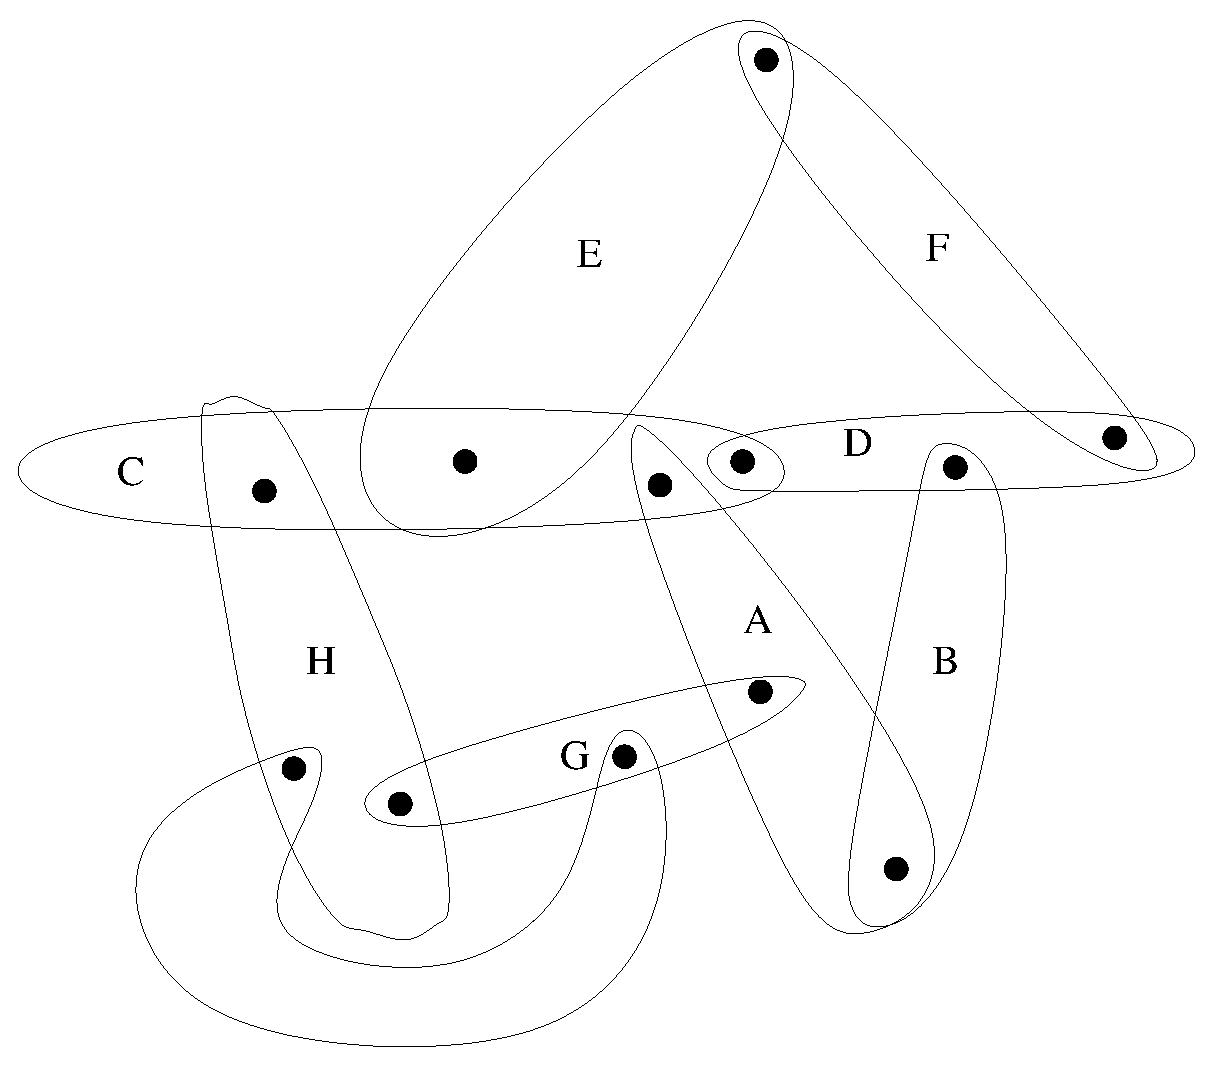
\includegraphics[width=\linewidth]{img/bodypin2}
    \caption{}
\end{subfigure}
%
\caption{(a) is a 1-dof body-pin graph. (b) is the corresponding body-bar graph explained in Definition \ref{def:body-pin}. (c) is the 1-dof DR-plan for the graph. In this case, to obtain an isostatic system, we would need to add a body and 2 pins to one of the nodes in the second level. (d) is the result of adding one such body to the bold-faced node.}
%
\end{figure*}

\begin{theorem}
\label{thm:1dofcase}
    Given a 1-dof body-pin or multi-triangle graph $G$ and corresponding 1-dof DR-plan $T$, there is a quadratic algorithm for the 1-dof optimal completion problem of Section \ref{sec:recomb} for body-pin and multi-triangle-pin graphs.
\end{theorem}

\begin{proof}
    Suppose we are given a body-pin graph and its corresponding body-bar graph $G$ and have obtained the 1-dof DR-plan $T$. Each node of $T$ will then be a vertex maximal proper 1-dof sub-graph of $G$.

    To make the graph isostatic, we need only add one body and pin it to 2 other bodies. Doing so will cause $G$ to become $(3,3)$-tight. We choose the 2 bodies to pin to by choosing a node $b$ in $T$ and looking at its children. From Observation \ref{rem:1dofcanon}, we know that the children can only be joined by a single pin or a sub-graph. We pin the new body to bodies in two separate children. Doing so will ensure that all children of $b$ will have 1-dof and all ancestors of $b$ (including $b$) will now be isostatic.

    % Then, we can form a valid isostatic DR-plan $T_b$ from $T$. In $T_b$, $fanin(b)$is the number of leaves in the subtree rooted at $b$ because no child of $b$ in $T$ is isostatic. Similarly, for any other node $w$ that is an ancestor of $b$, $fanin(w)$ is the the number leaf nodes in the tree rooted at $w$, excluding the subtree constaining $b$, plus 1 (for the node leading to $b$).  Then, for any node $b$ that we choose, $T_b$ is a valid DR-plan. The size of $T_b$ will just be the maximum fanin of all nodes in $T_b$. Thus, if we want to minimize the size of our DR-plan, we simply need to take the $b$ that has the $T_b$ of smallest size.

    Such a pinning covers all possible ways of adding a new body. Assume we add a new body $b$ to our graph and pin it to $b_i$ and $b_j$ to make it isostatic. Then, there will be some lowest 1-dof node $v$ in $T$ such that $b_i$ and $b_j$ appear in $v$. Thus, pinning $v$ in the manner described yields an equivalent isostatic DR-plan to pinning $b$ to $b_i$ and $b_j$.

    For each node $b$, we assign a size of the $T_b$ denoted $|T_b|$. $|T_b| = \displaystyle\max_{v \in T_b} fanin(v)$. We are looking for $b$ that minimizes $|T_b|$. Denote the sub-tree of $T$ rooted at $v$ by $T^v$ and the number of leaves in a tree $T$ by $nl(T)$. Note that $fanin(b)= nl(T^b)$ because no descendant of $b$ is isostatic. Similarly, for any ancestor $w$ of $b$, $fanin(w) = nl(T^w)-nl(T^{b'})+1$, where $b'$ is the child leading to $b$. All other nodes are not isostatic and so have no fanin.

    % Then, we can form a valid isostatic DR-plan $T_b$ from $T$. In $T_b$, $b$'s children are now all of the leaf nodes of the subtree rooted at $b$ because no child of $b$ in $T$ is isostatic. Similarly, for any other node $w$ that is an ancestor of $b$, $w$'s children will be the node that leads to $b$, denoted $b'$, along with all of the other leaf nodes in the tree rooted at $w$, excluding $b'$. Then, for any node $b$ that we choose, $T_b$ is a valid DR-plan. The size of $T_b$ will just be the maximum fanin of all nodes in $T_b$. Thus, if we want to minimize the size of our DR-plan, we simply need to take the $b$ that has the $T_b$ of smallest size.

    The node we need to pin will always be the deepest nontrivial node of some path in $T$. Suppose we chose to pin a node $b$ that has a nontrivial child $v$. Then, $fanin_b(b) = nl(T^b) = nl(T^v) + n$, where $n$ is essentially the number of leaves between $b$ and $v$. If we had instead chosen to pin $v$, then $fanin_v(b) = nl(T^b) - nl(T^{b'}) + 1 \leq fanin_b(v)$. And for each ancestor $w$ of $b$, $fanin(w)$ is unchanged, meaning $|T_v| \leq |T_b|$. Thus we only have to check the deepest non-trivial nodes.

    Running this algorithm in a brute force fashion is quadratic in the number of bodies of our given body-pin system.

    For the multi-triangle pin graphs, we can do the same thing except we need to add a single triangle to one of the nodes to cause it to become isostatic.
    % Don't leave a blank line between last paragraph and end!
    % For the 2-dof case, we can do something very similar, except instead of pinning a single body 2 times to a node, we can pin another body 2 times to a node. These can be the same node, and if it is the same node, we can find a wellconstrained DR-plan in quadratic time, we would just be doing the same thing as the 1-dof case.
\end{proof}

\begin{observation}
    For the 2-dof case, if a similar statement to Remark \ref{rem:1dofcanon} can be made, then Theorem \ref{thm:1dofcase} is true for 2-dof as well.
\end{observation}

\begin{proof}
    The only difference from the 1-dof case is that now we need to remove 2-dof from our graph. We build a 2-dof DR-plan $T$. Like above, we need to add a body and 2 pins to 2 nodes now to get to isostatic.

    Suppose we pin 2 distinct nodes $v_i$ and $v_j$. Then, there will be some common ancestor $a$ of $v_i$ and $v_j$. Then, in $T_{v_i,v_j}$, $fanin_{v_i,v_j}(a) = nl(T^a)$. However, if we chose to pin one of $v_i$ and $v_j$ twice, then $fanin_v(a) = nl(T^a) - nl(T^{a'}) +1$ . Thus $fanin_v(a)' \leq fanin_{v_i,v_j}(a)$. All ancestors of $a$ are unchanged. So $|T_v| \leq |T_{v_i,v_j}|$.

    So, we will always end up pinning a single node twice. Hence, we can run the same algorithm as the 1-dof case and just pin twice instead of once.
\end{proof}

\begin{observation}
    While the proof for Theorem \ref{thm:1dofcase} gives us a DR-plan with minimum fanin, we did not consider the algebraic complexity of realizing the DR-plan. If that is preferred, we can no longer only consider the deepest nodes.
\end{observation}

\begin{proof}
    An isostatic graph has 3 parameters that define it (in terms of coming up with a realizaiton). These are the Euclidean motions. A 1-dof graph can be seen as essentially having 4 parameters: the 3 Euclidean motions and whatever degree of freedom it has. A 2-dof has 5 parameters, and so on. These paramters denote the algebraic complexity of giving a realization for the graphs.

    Thus, say we have a $T$ as described in the proof for Theorem \ref{thm:1dofcase}. When we pin a node $b$, we will have the same structure as before. Suppose we are looking at an isostatic node $v$ after pinning $b$. Then, the children of $v$ (except one if $v \neq b$) will be 1-dof. The complexity for that node is then just that of solving each of its children. In general then, the number of parameters for that node will be $np(v) = 4nc_1(v)+3$, if $v \neq b$ and $np(b) = 4nc_1(b)$, where $nc_k(v)$ is the number of $k$-dof children of $v$.

    Now if we want to minimize the algebraic complexity, we need to minimize the maximum $np(v)$ for any node $v$. In this case, we cannot always just choose the node furthest down the tree to pin because it could have many children. SO we will have to try pinning all nodes to see which gives the lowest algebraic complexity. This is still quadratic for the 1-dof case.

    For the 2-dof case, there are more cases to consider. If we pin the same node twice as above, we have $np(v) = 5nc_2(v)+3$ for any ancestor $v \neq b$ and $np(b) = 5nc_2(b)$. If we pin a node $v$ and one of its ancestors $v'$, then any nodes between $v'$ and $v$ will be 1-dof, any nodes above $v'$ will be isostatic, and nodes below $v$ will be 2-dof. Note that solving $v'$ will result in solving $v$. Then, we need to consider nodes above and includiing $v'$ in our complexity. $np(v') = 5nc_2(v') + 4$ and $np(a) = 3 + 5nc_2(a)$ for $a$ an ancestor of $v'$. The only remaining case will be if we pin two nodes that are not descendent/ancestor. the only change from the previous case will be that for the lowest common ancestor of the nodes $v'$, $np(v') = 2*4+5nc_2(v')$. For any ancestor $a$ of $v'$, we still have $np(a) = 3 + 5nc_2(a)$.

    Like the 1-dof case, we again cannot just choose the nodes deepest in the tree to pin. However, we cannot also assume pinning one node twice will give us the best algebraic complexity. Hence, we will need to check each pair of node to pin. This makes our brute-force algorithm $O(b^3)$, where $b$ is the number of bodies.
\end{proof}

\begin{openproblem}
    What is the complexity of the optimal completion problem when there are more than 2-dof. For higher number of dofs, the $(k,l)$ characterization is no longer matroidal.
\end{openproblem}
